\documentclass[12pt,twoside, a4paper, twocolumn]{article}
\usepackage[utf8]{inputenc}
\usepackage[brazil]{babel}
\usepackage[margin = 0.5in]{geometry}
\usepackage{amsmath}
\usepackage{amsthm}
\usepackage{amssymb}
\usepackage{amsthm}
\usepackage{setspace}
\usepackage[americanvoltages,fulldiodes,siunitx]{circuitikz}
\usepackage{lipsum}
\usepackage{pgfplots}
\usepackage{ifthen}
\usepackage{adjustbox}
\usepackage[section]{placeins}
\usepackage{hyperref}
\usepackage{graphicx}
\pgfplotsset{compat=newest}
\graphicspath{ {./images/} }
%  #1 color - optional #2 x_0 #3 y_0 #4 x_f #5 y_f #6 name - optional  #7 true if adding lines to axis
\newcommand{\drawvector} [9] [color=cyan] {
  \draw[line width=1.5pt,#1,-stealth](axis cs: #2, #3)--(axis cs: #4, #5) node[anchor=south west]{$#6$};
 \ifthenelse{\equal{#7}{true}}{
  \draw[line width=1pt,#1, dashed](axis cs: #4, #5)--(axis cs: #4, 0) node[anchor= north west]{$#8$};
  \draw[line width=1pt,#1, dashed](axis cs: #4, #5)--(axis cs: 0, #5) node[anchor=south east]{$#9$};
  }
  {}
}
\newcommand\deriv[2]{\frac{\mathrm d #1}{\mathrm d #2}}
\title{Terceiro Relatório de Física Experimental 2}
\author{Henrique da Silva \\ hpsilva@proton.me}
\date{\today}
\pgfplotsset{width = 10cm, compat = 1.9}
\begin{document}
\maketitle
\pagenumbering{gobble}
\newpage
%pagenumbering{roman}
\tableofcontents
\newpage

\section{Introdução}

\paragraph*{Neste relatório, vamos discutir o capacitor. E como ele se comporta sobre a ação de correntes diretas e alternadas.}

\paragraph*{Todos arquivos utilizados para criar este relatório, e o relatório em si estão em:  \url{https://github.com/Shapis/ufpe_ee/tree/main/4th semester/}}


\section{Funcionamento basico de um osciloscopio}

\subsection{Comparando as ondas geradas com a visualização no osciloscópio}

\subparagraph*{Fizemos isto e observamos o comportamento senoidal e quadratico respectivamente das ondas na tela do osciloscópio.}

\subsection{Gráficos das ondas observadas}

\subsubsection{Grafico da tensão $V_{ad}$ pelo tempo em milisegundos no acoplamento AC}

\begin{tikzpicture}
    \begin{axis}[
            ylabel={Tensao $V$},
            xlabel={Tempo $ms$},
            xmin = 0, xmax = 10,
            ymin = -4, ymax = 5.0,
            xtick distance = 1,
            ytick distance = 1,
            grid = both,
            minor tick num = 1,
            major grid style = {lightgray},
            minor grid style = {lightgray!25},
            width = \textwidth,
            height = 0.5\textwidth]
        \addplot[
            domain = 0:10,
            samples = 400,
            smooth,
            thick,
            blue,
        ] {1 + 3 * cos(deg(2*pi*0.5* x))};
    \end{axis}
\end{tikzpicture}

\subsubsection{Grafico da tensão $V_{ad}$ pelo tempo em milisegundos no acoplamento DC}

\begin{tikzpicture}
    \begin{axis}[
            ylabel={Tensao $V$},
            xlabel={Tempo $ms$},
            xmin = 0, xmax = 10,
            ymin = -4, ymax = 5.0,
            xtick distance = 1,
            ytick distance = 1,
            grid = both,
            minor tick num = 1,
            major grid style = {lightgray},
            minor grid style = {lightgray!25},
            width = \textwidth,
            height = 0.5\textwidth]
        \addplot[
            domain = 0:10,
            samples = 400,
            smooth,
            thick,
            blue,
        ] {1 };
    \end{axis}
\end{tikzpicture}


\clearpage
\subsubsection{Gráfico da tensão $V_{bd}$ pelo tempo em milisegundos no acoplamento AC}

\begin{tikzpicture}
    \begin{axis}[
            ylabel={Tensao $V$},
            xlabel={Tempo $ms$},
            xmin = 0, xmax = 10,
            ymin = -4, ymax = 5.0,
            xtick distance = 1,
            ytick distance = 1,
            grid = both,
            minor tick num = 1,
            major grid style = {lightgray},
            minor grid style = {lightgray!25},
            width = \textwidth,
            height = 0.5\textwidth]
        \addplot[
            domain = 0:10,
            samples = 400,
            smooth,
            thick,
            blue,
        ] {1 + 2.1 * cos(deg(2*pi*0.5* x))};
    \end{axis}
\end{tikzpicture}

\subsubsection{Grafico da tensão $V_{bd}$ pelo tempo em milisegundos no acoplamento DC}

\begin{tikzpicture}
    \begin{axis}[
            ylabel={Tensao $V$},
            xlabel={Tempo $ms$},
            xmin = 0, xmax = 10,
            ymin = -4, ymax = 5.0,
            xtick distance = 1,
            ytick distance = 1,
            grid = both,
            minor tick num = 1,
            major grid style = {lightgray},
            minor grid style = {lightgray!25},
            width = \textwidth,
            height = 0.5\textwidth]
        \addplot[
            domain = 0:10,
            samples = 400,
            smooth,
            thick,
            blue,
        ] {1};
    \end{axis}
\end{tikzpicture}

\clearpage
\subsubsection{Gráfico da tensão $V_{cd}$ pelo tempo em milisegundos no acoplamento AC}

\begin{tikzpicture}
    \begin{axis}[
            ylabel={Tensao $V$},
            xlabel={Tempo $ms$},
            xmin = 0, xmax = 10,
            ymin = -4, ymax = 5.0,
            xtick distance = 1,
            ytick distance = 1,
            grid = both,
            minor tick num = 1,
            major grid style = {lightgray},
            minor grid style = {lightgray!25},            width = \textwidth,
            height = 0.5\textwidth]
        \addplot[
            domain = 0:10,
            samples = 400,
            smooth,
            thick,
            blue,
        ] { 1.25 * cos(deg(2*pi*0.5* x))};
    \end{axis}
\end{tikzpicture}

\subsubsection{Gráfico da tensão $V_{cd}$ pelo tempo em milisegundos no acoplamento DC}

\begin{tikzpicture}
    \begin{axis}[
            ylabel={Tensao $V$},
            xlabel={Tempo $ms$},
            xmin = 0, xmax = 10,
            ymin = -4, ymax = 5.0,
            xtick distance = 1,
            ytick distance = 1,
            grid = both,
            minor tick num = 1,
            major grid style = {lightgray},
            minor grid style = {lightgray!25},
            width = \textwidth,
            height = 0.5\textwidth]
        \addplot[
            domain = 0:10,
            samples = 400,
            smooth,
            thick,
            blue,
        ] {0};
    \end{axis}
\end{tikzpicture}

\clearpage

\subsection{Medindo $V_{ab}$ , $V_{bd}$, e $V_{cd}$}

\subparagraph*{Não podemos fazer estas medições diretamente pois estariamos alterando o circuito se encaixassem o osciloscópio nos pontos AB, BD, e CD respectivamente.}

\subsection{Papel do capacitor}

\subparagraph*{Este está "bloqueando" a passagem da corrente direta. Isto acontece porque a medida que a corrente direta carrega o capacitor, a tensão nos terminais do capacitor se iguala. }
\subparagraph*{Quando o capacitor está completamente carregando, as tensões nos seus terminais ficam igual, e não há passagem de corrente.}

\subsection{Equações das tensões}

\begin{center}
    \begin{tabular}{ |ccc| }
        \hline
        $AC: V_{ad}$ & $\rightarrow$ & V = 1 + 3cos(2pi*500*t)   \\
        $DC: V_{ad}$ & $\rightarrow$ & V = 1                     \\
        $AC: V_{bd}$ & $\rightarrow$ & V = 1 + 2.1cos(2pi*500*t) \\
        $DC: V_{bd}$ & $\rightarrow$ & V = 1                     \\
        $AC: V_{cd}$ & $\rightarrow$ & V = 1.25cos(2pi*500*t)    \\
        $DC: V_{cd}$ & $\rightarrow$ & V = 0                     \\
        \hline
    \end{tabular}
\end{center}




\subsection{Medicoes no multimetro}

\subparagraph*{$DC = 0.855V$ e $AC = 2.069V$}

\subparagraph*{Indicando que estamos lidando com medições rms}

\subsection{Diferenca entre valores medios e RMS}

\subparagraph*{Valores RMS nós levamos em consideração a raiz dos quadrados de todos valores. O que faz com que correntes alternadas somem ao valor. }

\subparagraph*{Já valor médio, o caso da corrente alternada somaria como 0. Já que há o mesmo número de valores positivos que negativos}

\subparagraph*{O caso no qual rms = valor médio será o caso no qual não há componente de corrente alternada no sistema.}

\clearpage

\section{Carga e descarga de um capacitor}

\subsection{Gráfico de Tensão sobre tempo da carga e descarga de um capacitor sob ação de uma fonte de tensão quadrática}

\begin{tikzpicture}
    \begin{axis}[
            ylabel={Tensao $V$},
            xlabel={Temp $s$ em ms},
            xmin = 0, xmax = 9,
            ymin = -1, ymax = 5.0,
            xtick distance = 1,
            ytick distance = 1,
            grid = both,
            minor tick num = 1,
            major grid style = {lightgray},
            minor grid style = {lightgray!25},
            width = \textwidth,
            height = 0.5\textwidth]
        \addplot[
            domain = 0:1.5,
            samples = 400,
            smooth,
            thick,
            blue,
        ] {4*(1-e^-x/0.3)};
        \addplot[
            domain = 1.5:3,
            samples = 400,
            smooth,
            thick,
            blue,
        ] {4*e^-(x-1.5)/0.3};
        \addplot[
            domain = 3:4.5,
            samples = 400,
            smooth,
            thick,
            blue,
        ] {4*(1-e^-(x-3)/0.3)};
        \addplot[
            domain = 4.5:6,
            samples = 400,
            smooth,
            thick,
            blue,
        ] {4*e^-(x-4.5)/0.3};
        \addplot[
            domain = 6:7.5,
            samples = 400,
            smooth,
            thick,
            blue,
        ] {4*(1-e^-(x-6)/0.3)};
        \addplot[
            domain = 7.5:9,
            samples = 400,
            smooth,
            thick,
            blue,
        ] {4*e^-(x-7.5)/0.3};

    \end{axis}
\end{tikzpicture}

\subparagraph*{Neste ponto seria interessante notar que a constante de tempo $RC = \tau$ é igual a cinco vezes o tempo de decaimento ou de subida de tensão do capacitor. ou seja. $3ms/10$ ou seja. $0.3ms$}

\clearpage

\subsection{Tabelas de estimativa}


\paragraph*{Tabela1: Carga}
\begin{center}
    \begin{tabular}{ |cc| }
        \hline
        $Tensao, V_{c} \pm 0.2V$ & $Tempo, t \pm 0.1ms$ \\
        $2.5 V$                  & 0.3 ms               \\
        $3.5 V$                  & 0.6 ms               \\
        $3.8 V$                  & 0.9 ms               \\
        $3.9 V$                  & 1.2 ms               \\
        $4.0 V$                  & 1.5 ms               \\
        \hline
    \end{tabular}
\end{center}



\paragraph*{Tabela1: Descarga}
\begin{center}
    \begin{tabular}{ |cc| }
        \hline
        $Tensao, V_{c} \pm 0.2V$ & $Tempo, t \pm 0.1ms$ \\
        $1.5 V$                  & 0.3 ms               \\
        $0.5V$                   & 0.6 ms               \\
        $0.2 V$                  & 0.9 ms               \\
        $0.1 V$                  & 1.2 ms               \\
        $0.0 V$                  & 1.5 ms               \\
        \hline
    \end{tabular}
\end{center}

\subsection{Gráficos das tabelas acima}

\begin{adjustbox}{scale=0.70}
    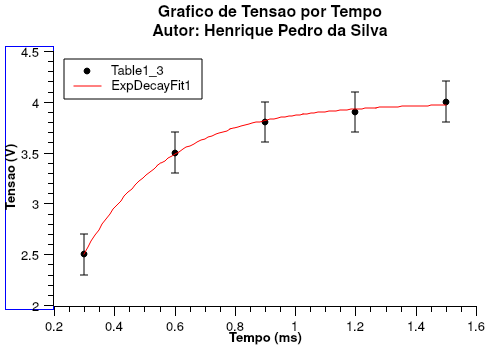
\includegraphics{Graph2.png}
\end{adjustbox}

\begin{adjustbox}{scale=0.70}
    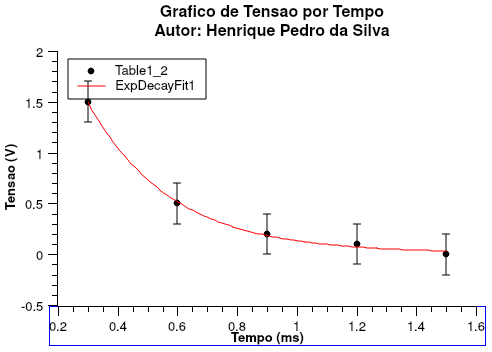
\includegraphics{Graph3.png}
\end{adjustbox}

\subparagraph*{Pelo fit feito pelo SciDAVis estimamos um $\tau$ de $0.27 \pm 0.07 ms$}

\subparagraph*{Que é coerente com o estimado visualmente com o $tau = 0.3ms$ que foi estimado visualmente no item (3.1).}

\subparagraph*{Interessantemente a amplitude estimada pelo fit do SciDAVis foi de $4.4 \pm 0.4V$, quando visualmente vemos que esta eh bem proxima de $4$ }

\subparagraph*{Isto indica que a estimativa visual foi superestimada em média.}

\subparagraph*{Para conseguir a Capacitancia vamos partir de:}

\begin{equation}
    \begin{aligned}
        RC & = \tau           \\
        C  & = \frac{\tau}{R}
    \end{aligned}
\end{equation}

\subparagraph*{Resolvendo esta conta com os valores encontrados acima, e derivando parcialmente para conseguir os erros isto nos dá:}

\begin{equation*}
    C = (2.5  \pm 0.8) * 10^{-8} F
\end{equation*}

\subsection{Discuta os resultados:}

\subparagraph*{Eu estou achando um pouco estranho um resultado tão baixo de capacitancia, estou sobre a impressão que houve algum erro de conversão de unidade mas não estou conseguindo identificá-lo.}

\subparagraph*{Mas no mais. Os resultados foram dentro do esperado, a estimativa a partir do SciDAVis acrescentou uma nova fonte de erro, mas manteve o resultado de $tau$ dentro do esperado.}

\subsection{Invertendo capacitor e resistor}

\subparagraph*{Neste caso o que vamos medir é a tensão no resistor, a medida que o capacitor é carregado e descarregado. Vamos ter um gráfico do oposto do que está acontecendo com a tensão do capacitor.}

\clearpage

\begin{tikzpicture}
    \begin{axis}[
            ylabel={Tensao $V$},
            xlabel={Temp $s$ em ms},
            xmin = 0, xmax = 9,
            ymin = -5, ymax = 5.0,
            xtick distance = 1,
            ytick distance = 1,
            grid = both,
            minor tick num = 1,
            major grid style = {lightgray},
            minor grid style = {lightgray!25},
            width = \textwidth,
            height = 0.5\textwidth]
        \addplot[
            domain = 0:1.5,
            samples = 400,
            smooth,
            thick,
            blue,
        ] {4*(e^-x/0.3)};
        \addplot[
            domain = 1.5:3,
            samples = 400,
            smooth,
            thick,
            blue,
        ] {4*(1-e^-(x-1.5)/0.3)-4};
        \addplot[
            domain = 3:4.5,
            samples = 400,
            smooth,
            thick,
            blue,
        ] {4*(e^-(x-3)/0.3)};
        \addplot[
            domain = 4.5:6,
            samples = 400,
            smooth,
            thick,
            blue,
        ] {4*(1-e^-(x-4.5)/0.3)-4};
        \addplot[
            domain = 6:7.5,
            samples = 400,
            smooth,
            thick,
            blue,
        ] {4*(e^-(x-6)/0.3)};
        \addplot[
            domain = 7.5:9,
            samples = 400,
            smooth,
            thick,
            blue,
        ] {4*(1-e^-(x-7.5)/0.3)-4};

    \end{axis}
\end{tikzpicture}



\end{document}